\documentclass{nascproject}
\usepackage{tikz}
\usepackage{tabularx}
\usepackage{pgfgantt}
\usepackage{pgfgantt}
\usepackage{lscape}
\usepackage{multirow}
\usepackage{colortbl}
\usepackage{lscape} % Optional: for landscape orientation

\usepackage{geometry}
\geometry{a4paper, total={6in, 9in}}
\usetikzlibrary{positioning, shapes}
\usepackage[T1]{fontenc}
\usepackage{geometry}
\title{RESULT ANALYSIS SYSTEM}
\team{\textbf{Aiswarya V }\\ \textbf{Anjana A}}
\author{Anjana A}
\begin{document}
\maketitle

\makecert

\newpage
%\thispagestyle{plain}
\pagenumbering{roman}
\setcounter{page}{1}
\newgeometry{top=4cm,bottom=0.1cm}
\renewcommand\abstractname{ABSTRACT}
\begin{abstract}
\vspace{5cm}

The Result Analysis System offers a streamlined and automated approach to address the essential task of monitoring and evaluating the academic performance of students within academic institutions. Manual methods for this purpose are not only time-consuming but also prone to human errors. This system provides an innovative solution that brings numerous advantages.

Enhanced Accuracy and Efficiency: By automating the result analysis process, this system significantly reduces the margin for errors that can occur during manual assessments. It ensures that academic evaluations are consistently accurate and efficient.

Improved Teacher-Student Communication: The system promotes better communication between teachers and students. This transparent communication fosters a constructive learning environment.

Empowering Educators: Teachers benefit from this system as well. They can conveniently upload university exam results, and the system promptly generates comprehensive reports. These reports allow teachers to evaluate their own teaching methods and better understand student outcomes. Armed with this data, educators can make informed decisions to refine their teaching strategies and enhance the learning experience.

In conclusion, the Result Analysis System is a valuable tool for academic institutions, offering not only efficiency and accuracy but also improved communication and empowerment for both teachers and students. It ushers in a new era of data-driven decision-making in education, ultimately leading to the continuous improvement of teaching and learning processes.
\end{abstract}


\newpage
%\thispagestyle{plain}
\renewcommand\abstractname{ACKNOWLEDGMENT}
\begin{abstract}
\vspace{5cm}
I would like to place on record my sincere thanks to all those who have contributed to the successful completion of my project. I express my gratitude to the Mr. Mithun A. V., Assistant Professor, Department of Computer Science for rendering me all the facilities for the successful completion and presentation of my project. I also thank all the faculties of the Department of Computer Science Department for their wholehearted co-operation and guidance in completeing my project successfully. Finally, we thank our family and  friends who contributed to the successful fulfillment of this project.
\vspace{1cm}
\begin{flushright}
Aiswarya V
Anjana A
\end{flushright}
\end{abstract}
\newpage

\restoregeometry
\tableofcontents
\newpage

\cleardoublepage
\addcontentsline{toc}{chapter}{\listfigurename}
\listoffigures
\newpage

\cleardoublepage
\addcontentsline{toc}{chapter}{\listtablename}
\listoftables
\newpage
\pagestyle{fancy}


\chapter{INTRODUCTION}
\pagenumbering{arabic}
\setcounter{page}{1}
\renewcommand{\baselinestretch}{1.50}
\section{Overview}

Academic institutions face the critical task of assessing and monitoring their students academic progress, a process that, when performed manually, can be both time-consuming and prone to errors. To address these challenges, the Result Analysis System offers a centralized and automated solution.

In our system, when the University publishes results, it empowers departmental teachers to effortlessly upload students' corresponding results. Subsequently, the system generates a multitude of insightful analyses. These tasks involve identifying top-performing students each semester, conducting in-depth single-subject analyses, evaluating individual student performance, and examining results on a semester-by-semester basis.

Moreover, the system provides an advanced search feature for enhanced accessibility. Any teacher or department within our college can access and benefit from these analyses. Additionally, our system facilitates access to the academic history of previous students who have studied at our institution, allowing retrieval of their results from any semester.
\subsection{Modules}
	There are 3 modules in our system.
  \begin{itemize}
  	\item Administrator
  	\item Teacher
  	\item Principal
  \end{itemize}


\subsection{Use Case Diagrams}
	Administrators are responsible for adding teachers, setting their passwords, and adding new courses(Figure\ref{usecase1}) . Currently, the addition of students is not within the system, as it is handled by the SMS (Student Management System) of your college. Teachers are responsible for uploading the results of students, and both teachers and the principal can view different result analyses.(Figure\ref{usecase2})
\begin{figure}
	\centering
	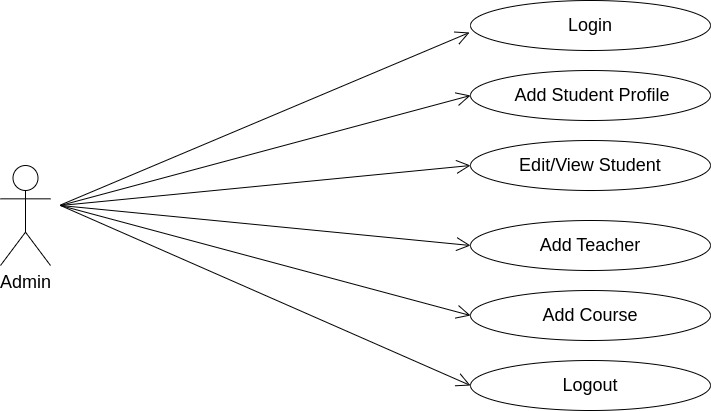
\includegraphics[width=1\linewidth]{usecase.jpg}
	\caption{Use case diagram of admin}
	\label{usecase1}
\end{figure}
\begin{figure}
	\centering
	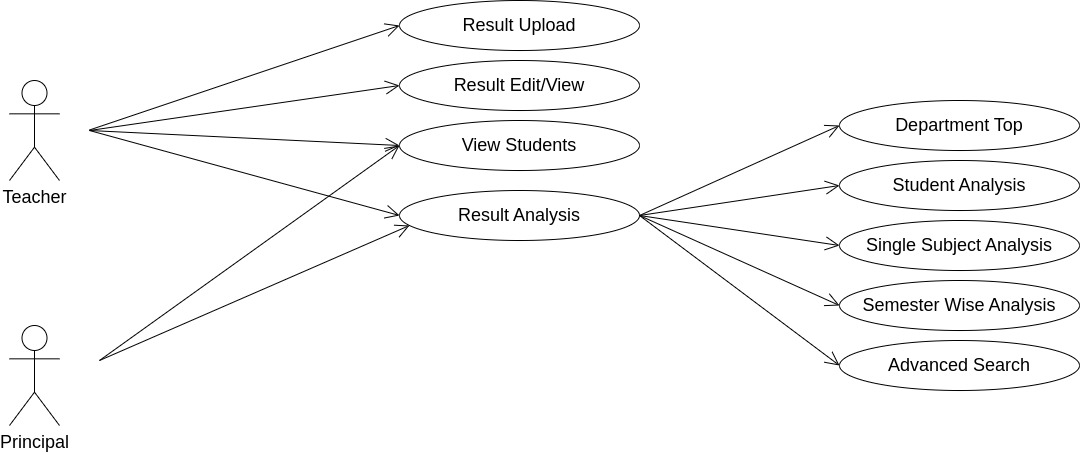
\includegraphics[width=1\linewidth]{usecase1.jpg}
	\caption{Use case diagram of teacher and principal}
	\label{usecase2}
\end{figure}
\section{Feasibility Study}
Feasibility study lets the developer for see the future of the project and the usefulness.
Feasibility study is a test of system proposed regarding its workability, impact on the
organization, ability to meet the needs and effective use of resources.

    \subsection {Technical Feasibility}
    The technical feasibility of Result Analysis System involves evaluating the system’s hard-
    ware and software requirements.\\
    
    \textbf{Hardware Requirements}
    \begin{itemize}
    	\item  Minimum RAM: 2GB
    	\item Processor: Pentium or equivalent with similar performance
    \end{itemize}
   
    
    \textbf{Software Requirements}
    \begin{itemize}
    	\item Operating System: Result Analysis System is designed to be platform-independent,
    	compatible with various operating systems such as Windows, macOS, and
    	Linux.
    	\item  Web Browser: The application runs on modern web browsers like Google
    	Chrome, Mozilla Firefox, Safari, and Microsoft Edge.
    	\item Programming Languages and Technologies:
    	\begin{itemize}
    		\item 	Frontend: Specify the frontend programming languages and technologies:
    		\begin{itemize}
    			\item HTML: For structuring web pages.
    			\item CSS: For styling and layout.
    			\item 	JavaScript: For interactive features and user interface enhancements.
    		\end{itemize}
    		\item 	Backend: Specify the backend programming languages and technologies:
    		\begin{itemize}
    			\item PHP: As the primary backend scripting language.
    			\item 	MySQL: As the relational database management system.
    		\end{itemize}
    	\end{itemize}	
   \end{itemize}
This system is a platform-independent, use MySQL for database, PHP as the server-side scripting language and html as user interface. Thus Result Analysis System is technically feasible.	
    \subsection{Economical Feasibility}
    The economic feasibility of the Result Analysis System is assessed by considering the financial aspects of the project. Our system proves to be a financially efficient choice for educational institutions and stakeholders, primarily due to the following factors:
    \begin{itemize}
    	\item Cost-Effective Solution: The Result Analysis System is designed to provide a cost-effective solution. It eliminates the need for expensive, proprietary software licenses, as it is built using open-source technologies. Educational institutions can implement and utilize the system without incurring licensing costs, promoting financial sustainability.
    	\item Scalability: Our system is engineered to scale seamlessly with the institution's needs. Whether there is an increase in the number of students or data volume, the system can adapt efficiently without demanding significant additional investments in infrastructure or operations.
    \end{itemize}
In conclusion, the Result Analysis System offers economic feasibility by optimizing resources, reducing costs, and promoting efficient result analysis within educational institutions. It stands as a financially prudent choice for institutions seeking to enhance their academic performance evaluation processes while maintaining fiscal responsibility.
    \subsection{Behavioural Feasibility}
    The Result Analysis System demonstrates strong behavioral feasibility, as it encompasses various aspects that enhance its ease of use and efficiency in operation. Here are the behavioral feasibility considerations for the system:
    \begin{itemize}
    	\item User-Friendly Interface: The system is designed with a user-friendly interface that ensures ease of use for teachers.
    	\item Reduced Human Effort: The new system significantly reduces the manual effort required for result analysis and reporting. It automates the process, minimizing the need for extensive human intervention. 
    	\item Historical Student Data Access: One of the unique features of the system is its ability to access previous student details. This capability allows educators and administrators to retrieve and analyze the performance history of students who have graduated or completed previous academic terms, providing valuable insights for continuous improvement.
    	
    	\item Versatile Analysis: The system offers the flexibility to perform various types of result analysis. Whether it's departmental analysis, student-level analysis, semester analysis, or single-subject analysis, the system provides the tools and data needed for comprehensive assessment.
    \end{itemize}
    
    In summary, the Result Analysis System's user-friendly features, reduced manual effort, accessibility, and versatile analysis options make it a valuable tool for improving academic performance evaluation in educational institutions.
   
   
   

\chapter{RELATED WORKS}
\section{System Analysis}
System analysis is a detailed study of the various operations performed by a system
and their relationship within and outside of the system. One aspect of analysis is defining the
boundaries of the system and determining whether or not a candidate system should consider
other related systems. During analysis, data are collected on the valuable file, decision points,and transactions handled by the present system. Once the analysis is completed the system
analyst has a firm understanding of what is to be done. System analysis and study has mainly
two parts. They are Existing System and Proposed System.
\subsection{Existing System}
The current system operates in a manual mode, demanding considerable effort and consuming a substantial amount of time. In this existing setup, when results are published, teachers are required to manually transcribe or document the results of each student. When it comes to conducting analyses, these tasks are also carried out manually, adding to the overall time and effort required for academic assessments.

\textbf{Disadvantages}
\begin{itemize}
	\item Time consuming
	\item High chance of error
	\item High manual effort
	\item Inadequate analysis
	\item Lack of different analyses
	\item Missing pre-student results
	\item Documentation is a challenging
\end{itemize}
\subsection{Proposed System}
The proposed system represents a significant departure from the current manual mode of operation. It introduces a streamlined and efficient approach to result analysis and academic assessments, leveraging modern technology to simplify processes.

In this proposed system, the need for manual transcription or documentation upon the publication of results is entirely eliminated. Teachers can effortlessly upload student marks and data directly into the system, greatly reducing the burden of manual data entry.

One of the primary advantages of the proposed system lies in its robust analytical capabilities. It offers a wide range of analytical tools and features that empower educators to conduct in-depth assessments with ease. These analyses encompass various aspects, including department-wise performance, student-specific insights, semester-wise trends, single-subject analyses, and advanced search functionality. This comprehensive suite of analytical components allows educators to gain deeper insights into student performance and academic trends.

\textbf{Advantages}
\begin{itemize}
	\item Time-efficient
	\item Reduced chance of error
	\item Minimized manual effort
	\item Enhanced analysis capabilities
	\item Diverse analysis options
	\item Comprehensive student performance history
	\item Streamlined documentation
\end{itemize}
\section{Requirement Elicitation and Analysis}
The analysis of requirements for the Result Analysis System commenced with a comprehensive gathering of information from various stakeholders, including students and Teachers. This initial phase aimed to collect all relevant data that would serve as the foundation for defining the system's requirements. The collected information underwent a thorough analysis to establish a precise and unambiguous understanding of the project's objectives, while also addressing any ambiguities or inconsistencies in the initial problem statement.
\subsection{Requirement Gathering}
For the requirement gathering process, a combination of methods was employed, including personal interviews and group discussions. These methods allowed for a holistic approach to gathering insights and needs for the project.\\
The following techniques were utilized:
\begin{itemize}
	\item Personal Interviews : Interviews were conducted with key stakeholders to identify the activities involved in the result analysis process, comprehend the limitations of the existing system, and discern the types of reports required.
	\item Checklists : Checklists were employed to systematically identify the areas within the result analysis system that required thorough analysis. This approach helped prioritize aspects of the system based on their significance. 
	\item Record Review : The examination of existing documentation played a pivotal role in understanding the standard operating procedures, forms, documents, and various reports utilized by the current system.
\end{itemize}
\chapter{METHODOLOGY}
\section{System Development}
The development of the Result Analysis System was executed using PHP, a server-side scripting language known for its versatility and web development capabilities. The user interface was crafted using HTML, CSS, and JavaScript to create an interactive and user-friendly front end. PHP, coupled with the Laravel framework, provided the foundation for the back-end logic. The development environment was established using tools such as Visual Studio Code, and version control was managed via Git.

\section{Database Design and Data Integration}
In our project, we recognized the importance of leveraging existing student data, which was already stored in the database of the college's Student Management System. This integration allowed us to build upon the foundation of pre-existing student details, eliminating the need to re-enter redundant data.To seamlessly integrate the Result Analysis System with the Student Management System's database, we extended the database schema to accommodate additional information related to courses and teachers.Admin of our project is responsible for entering course data including course name,course code,credit etc and teacher data include teacher name ,department into the database. By integrating with the existing Student Management System's database, we were able to build a seamless and comprehensive Result Analysis System while minimizing data duplication and maintaining data consistency across the college's information systems. This approach not only saved time and effort but also ensured that student, course, and teacher data remained accurate and synchronized.

We introduced an additional database table specifically designed to capture and manage mark data.It includes fields such studID,courseID and ce,ese marks.By creating this separate table, we ensured that teacher-entered marks were appropriately organized, securely stored, and easily accessible for analysis and reporting.
\section{User Feedback}
User feedback was an integral part of our methodology. We actively sought input from users, including teachers and administrators, at various stages of development.feedback sessions were conducted to gather insights into system usability and functionality.This feedback guided the refinement of system features and the user interface.
\section{Framework and Tool Selection}
In the process of developing a web app, we rely on a range of essential tools.
Such as:

• \textbf{Visual Studio Code} : It is an advanced code editor that offers features like debugging, syntax highlighting, intelligent code completion, snippets, code refactoring, and integrated Git support.

• \textbf{Git \& GitHub} : git and GitHub are fundamental tools in the realm of version control systems, essential for tracking changes across collections of files. These technologies enable effortless collaboration among developers collaborating on source code, with a focus on optimizing speed, maintaining data integrity, and supporting distributed, non-linear development.

• \textbf{phpMyAdmin} : phpMyAdmin is a web-based graphical interface used for managing MySQL and MariaDB databases. It simplifies database administration by providing a user-friendly interface accessible through web browsers. With phpMyAdmin, users can create, modify, and delete databases and tables, execute SQL queries, import and export data, and manage user privileges.


\chapter{DESIGN and IMPLEMENTATION}
\section{Architecture}
\subsection{Data Flow Diagram}
A Data Flow Diagram (DFD) is a graphical representation of the “flow” of data through
an information system.\\\\
\begin{itemize}
	\item Level 0 - Figure \ref{level_zero}
	\item Level 1 of process 1 - Figure \ref{level_one}
	\item Level 1 of process 2 - Figure \ref{level_teacher}
	\item Level 1 of process 3 - Figure \ref{level_prin}
\end{itemize}
\begin{figure}
	\centering
	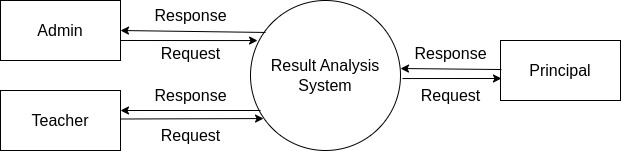
\includegraphics[width=1\linewidth]{level_zero.jpg}
	\caption{Level 0: DFD}
	
	\label{level_zero}
\end{figure}
\begin{figure}
	\centering
	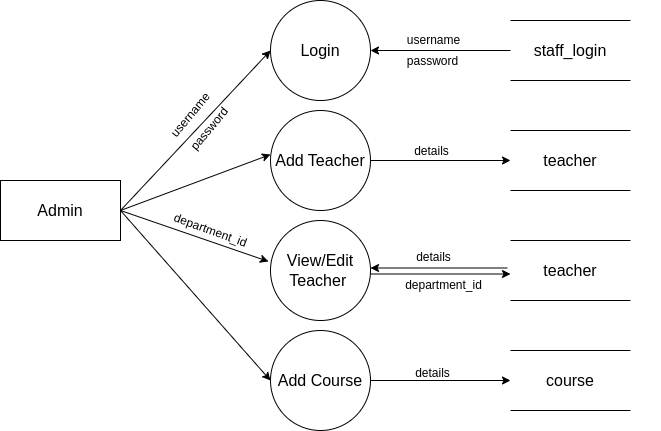
\includegraphics[width=1\linewidth]{level_admin.png}
	\caption{Level 1 of process 1: DFD}
	\label{level_one}
\end{figure}
\begin{figure}
	\centering
	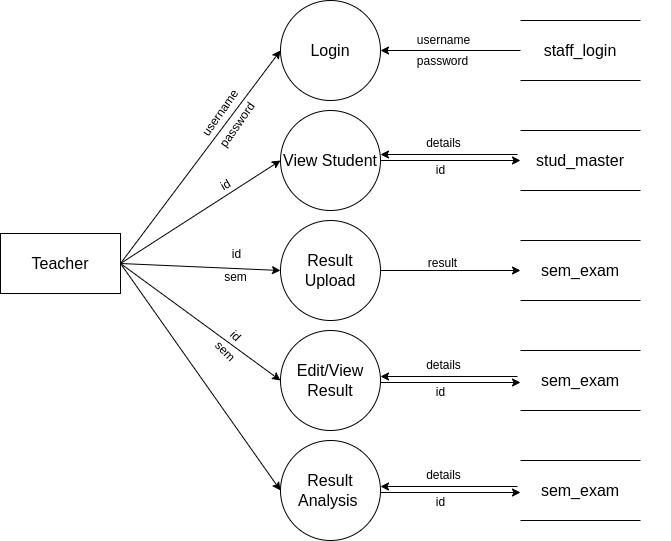
\includegraphics[width=1\linewidth]{level_teacher.jpg}
	\caption{Level 1 of process 2: DFD}
	\label{level_teacher}
\end{figure}
\begin{figure}
	\centering
	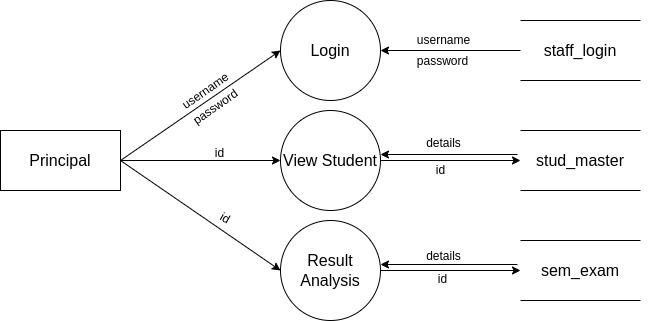
\includegraphics[width=1\linewidth]{level_p.jpg}
	\caption{Level 1 of process 3: DFD}
	\label{level_prin}
\end{figure}
\subsection{ER Diagram}
An entity-relationship diagram is a data modeling technique that creates a graphical
representation of the entities, and the relationships between entities, within an information
system. Figure \ref{er} represent our ER diagram.
\begin{figure}
	\centering
	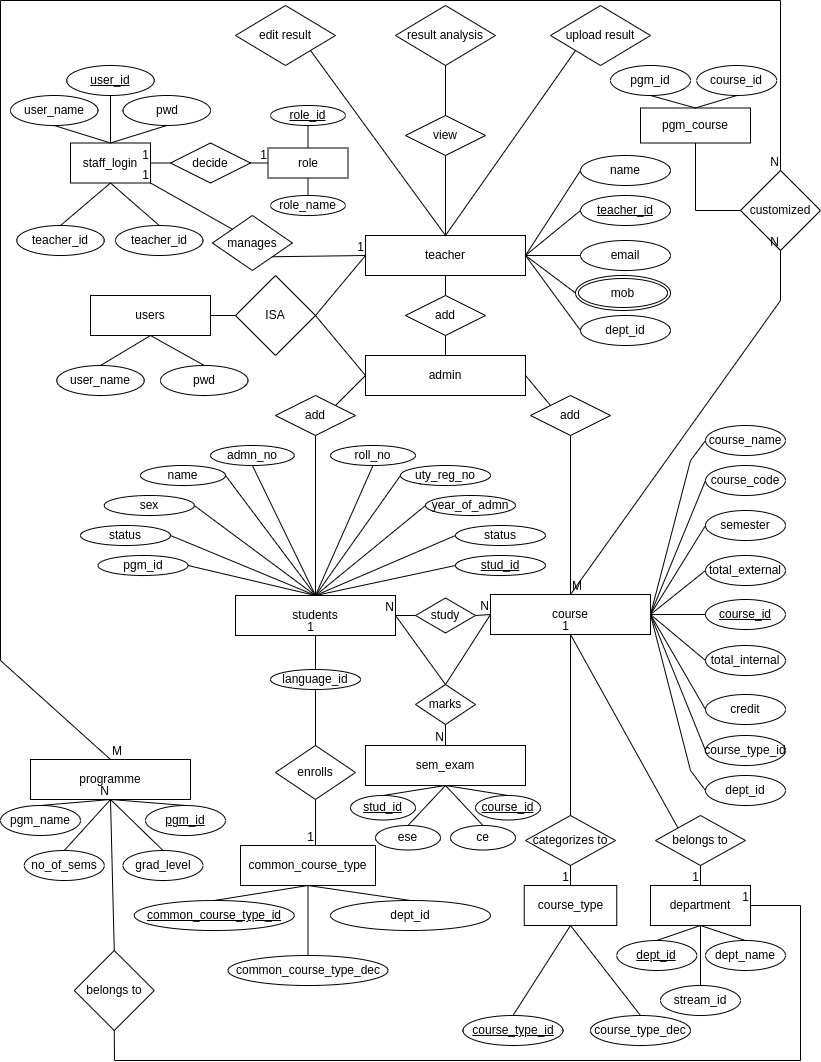
\includegraphics[width=1\linewidth]{er.png}
	\caption{ER daigram}
	\label{er}
\end{figure}
\subsection{Database Design}

\begin{itemize}
	\item Table Name : stud\textunderscore master (Table \ref{studmaster})
	
	Description : Details of students
\end{itemize}

	\begin{table}
		\centering
		\begin{tabular}{|c|c|c|}
			\hline
			\textbf{Column name}& \textbf{Data Type} &\textbf{Description} \\
			\hline
			stud\textunderscore id & int & id of student \\
			\hline
			roll\textunderscore no & int & roll no of student \\
			\hline
			uty\textunderscore reg\textunderscore no& int & register number of student \\
			\hline
			name & varchar(50) & name of student \\
			\hline
			year\textunderscore of\textunderscore admin& int & year of admission \\
			\hline
			sex & char(1) & sex\\
			\hline
			pgm\textunderscore id& int & programme \\
			\hline
			language\textunderscore id& int & second language \\
			\hline
		\end{tabular}
		\caption{Student Details}
		\label{studmaster}
	\end{table}
\begin{itemize}
	\item Table Name : course (Table \ref{course})
	
	Description : Details of papers
\end{itemize}
	
		\begin{table}
		\centering
		\begin{tabular}{|c|c|c|}
		
			\hline
		\textbf{Column name}& \textbf{Data Type} &\textbf{Description} \\
		\hline
		course\textunderscore id & int & id of course \\
		\hline
		course\textunderscore title & varchar(100) & course name \\
		\hline
		course\textunderscore code& varchar(12) & course code \\
		\hline
		lab\textunderscore theory & char(1) & lab/theory \\
		\hline
		course\textunderscore type\textunderscore id& int & course type \\
		\hline
	
		dept\textunderscore id& int & department \\
		\hline
		semester& int & semester \\
		\hline
		syllabus\textunderscore intro\textunderscore year& int & year of syllabus \\
		\hline
		credits & int & credit \\
		\hline
		total\textunderscore internal& int & total internal \\
		\hline
		total\textunderscore external& int & total external \\
		\hline
		\end{tabular}
		\caption{Course Details}
		\label{course}
	\end{table}
	\begin{itemize}
		\item 	Table Name : sem\textunderscore exam (Table \ref{semexam})
		
		Description : Result of students
	\end{itemize}

		\begin{table}
		\centering
		\begin{tabular}{|c|c|c|}
			\hline
			\textbf{Column name}& \textbf{Data Type} &\textbf{Description} \\
			\hline
			course\textunderscore id& int & course id \\
			\hline
			stud\textunderscore id& int & student id \\
			\hline
			ce& int & internal mark obtain \\
			\hline
			ese& int & external mark obtain \\
			\hline
		\end{tabular}
		\caption{Result of Students}
		\label{semexam}
	\end{table}


\section{Implementation}
	We gathered information for our project through personal interviews with teachers, checklists, previous analyses, and record reviews. During our research, we identified that manual analysis processes were time-consuming and prone to errors. As a result, we concluded that implementing our system within the college context would be a sensible solution. 
The proposed system has been developed using PHP for the front-end, with HTML, CSS, and JavaScript utilized for design and user interface components. MySQL is employed as the back-end database. We provided sample data for testing our code and identified an issue where marks can be uploaded exceeding the maximum allowed mark. This testing process has been crucial in validating our project and finding a solution to the problem. Testing is indeed a vital step in the development process to ensure the correctness and reliability of our system.

	In figure \ref{timeline}, we can observe the comprehensive depiction of our project's growth and timeline chart, providing a visual representation of its evolution over time. 
	


	\begin{table}[h]
		\centering
		\begin{tabular}{|c|c|c|c|c|c|}
			\hline
			& Mar & Jun & Jul & Aug & Sep \\
			\hline
			Planning & \cellcolor{gray!30} & \cellcolor{gray!30} & & &  \\
			\cline{1-2}
			Design & & \cellcolor{gray!30} & \cellcolor{gray!30} & &  \\
			\cline{1-4}
			Coding & & & & \cellcolor{gray!30} & \cellcolor{gray!30}  \\
			\cline{1-6}
			Testing & & & & & \cellcolor{gray!30}  \\
			
		
		\end{tabular}
	\caption{TimeLine Chart}
	\label{timeline}
	\end{table}



\chapter{TESTING}
Testing is a critical phase to ensure that the system functions correctly and meets its intended objectives
\section{Testing Strategy}
\subsection{System Testing}
System testing evaluates the entire system as a whole, including end-to-end functionality. 
\subsection{Unit Testing}
Unit testing involves testing individual components and functions of the application to ensure they perform as expected. This stage includes checking the accuracy of mark uploads and data processing.
\subsection{Integration Testing}
Integration testing assesses the interactions between different modules and components of the system. We validate that data flows seamlessly between the teacher's mark upload interface and the analytical components of the web application.
\section{Test Cases}
In this section, we outline the test cases designed to evaluate the functionality of our Result Analysis System. Each test case focuses on specific aspects of the system, ensuring comprehensive coverage.
\subsection{Mark Upload Testing}
Test Case : Uploading Marks for Sample Students\\
Objective: To verify the accuracy and integrity of mark uploads.\\
Steps: Teachers upload marks for a sample set of students.\\
Expected Result: Marks are successfully uploaded, and the data is correctly processed.
\subsection{Department Top Analysis Testing}
Test Case : Department Top Analysis\\
Objective: To confirm that the system accurately identifies top-performing students within a department.\\
Steps: Analyze results to find the top students in a selected department.\\
Expected Result: The system correctly identifies the top students based on their marks.
\subsection{ Student wise Analysis Testing}
Test Case : Student-Specific Analysis\\
Objective: To validate the system's ability to provide individual student mark status analysis.\\
Steps: Access the individual student's profile for the chosen semester.\\
Expected Result: Accurate display of the student's analysis for the specified semester.\\
\subsection{Semester-wise Analysis Testing}
Test Case : Semester-wise Analysis\\
Objective: To ensure that the system can perform semester-wise analysis.\\
Steps: Select a specific semester and examine the performance data.\\
Expected Result: Accurate presentation of performance data for the chosen semester.
\subsection{Single Subject Analysis Testing}
Test Case : Single-Subject Analysis\\
Objective: To verify that the system provides in-depth analysis of a single subject's performance.\\
Steps: Select a subject and analyze the results.\\
Expected Result: Accurate presentation of performance insights for the chosen subject.
\subsection{ Advanced Search Testing}
Test Case : Advanced Search Functionality\\
Objective: To confirm the effectiveness of the advanced search feature.\\
Steps: Perform advanced searches using various criteria.\\
Expected Result: Return of relevant and accurate search results.\\

In the initial stage of the uploading process, the system inadvertently permitted the uploading of marks that exceeded the maximum allowable mark for a particular paper. This oversight had the potential to significantly distort the subsequent analysis. Recognizing this issue, we promptly addressed it by implementing a code modification. This modification now prevents the addition of marks that exceed the established maximum mark, ensuring the integrity and accuracy of the analysis process.That is when a user attempts to upload a mark above the maximum allowed mark, the system immediately provides a visual indication by highlighting the input box with a distinct red border (Figure\ref{testing}). This ensures that the marks stay within the specified limits and maintains data accuracy.
\begin{figure}
	\centering
	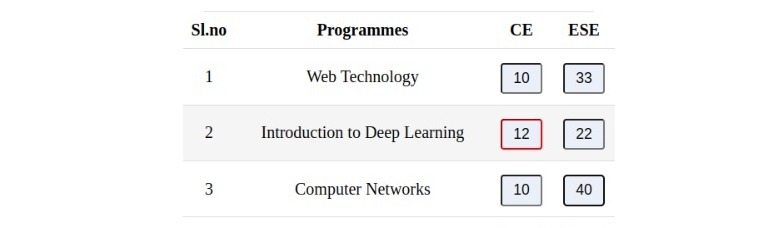
\includegraphics[width=1\linewidth]{testing.jpeg}
	\caption{Mark uploading error}
	\label{testing}
\end{figure}
\chapter{RESULTS AND DISCUSSION}
The Result Analysis System is a comprehensive software solution designed to streamline and enhance the academic performance evaluation process within educational institutions. The automation of result analysis has not only reduced manual effort but also improved the quality of evaluations. With consistent and reliable results, educators can make data-informed decisions to enhance the learning experience.The system's ability to conduct various types of analyses, such as departmental top analysis and historical data retrieval, offers a deeper understanding of academic performance trends. This information is invaluable for academic planning and decision-making.
\section{Results}
\subsection{Uploading result of students}
\begin{figure}
	\centering
	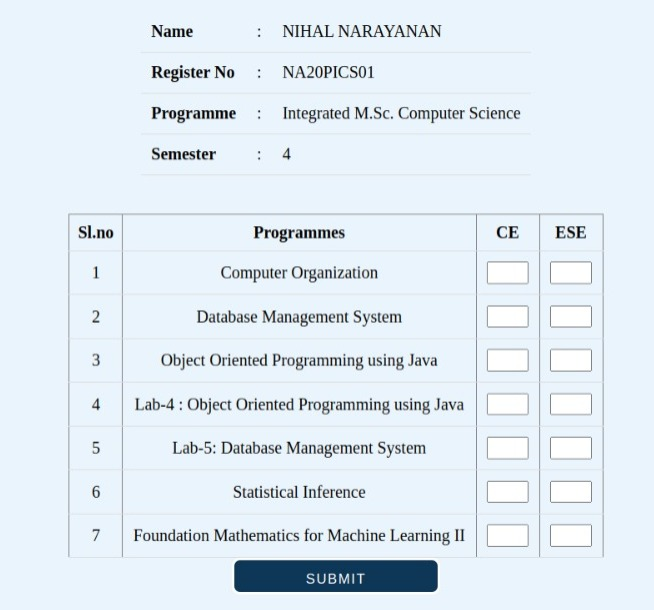
\includegraphics[width=1\linewidth]{upload1.jpeg}
	\caption{Uploading result}
	\label{upload}
\end{figure}
We have successfully implemented the capability to upload results for each student according to their papers in each semester (Figure \ref{upload}).

\subsection{Different types of analysis}
We have conducted various types of analysis, including departmental top analysis and semester-wise analysis, student analysis, single subject analysis etc.
\begin{figure}
	\centering
	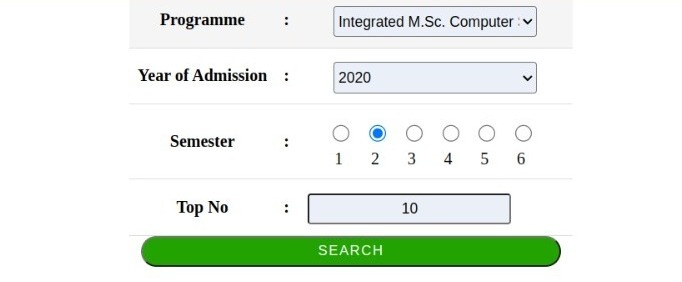
\includegraphics[width=1\linewidth]{dept_top.jpeg}
	\caption{Department top searching}
	\label{dept_top}
\end{figure}
In department top section, we get the top number of students in each semesters (Figure \ref{dept_top}).
\begin{figure}
	\centering
	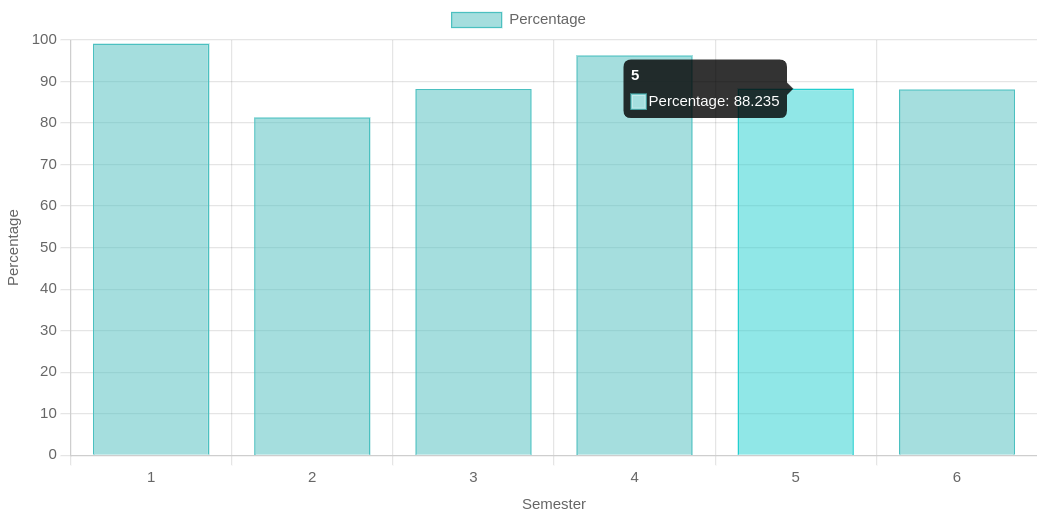
\includegraphics[width=1\linewidth]{bar_diagram.png}
	\caption{Bar diagram of a student based on semesters}
	\label{graph}
\end{figure}
In student analaysis, we include bar diagrams. Thus teachers can understand the growth of students(Figure \ref{graph}).
\begin{figure}
	\centering
	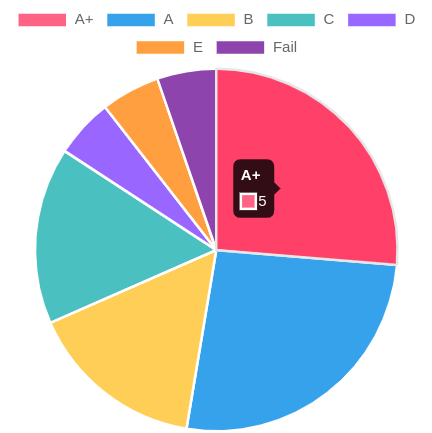
\includegraphics[width=0.5\linewidth]{pie1.png}
	\caption{Pie chart depicting the distribution of grades for a specific paper.}
	\label{pie}
\end{figure}
\section{Discussion}
The Result Analysis System is a development, in the field of evaluating performance in educational institutions. This system offers educators an efficient platform equipping them with tools to analyze student results comprehensively. Our Result Analysis System introduces an automated approach significantly enhancing the accuracy and effectiveness of result assessments. By eliminating the possibility of errors it establishes a foundation, for consistently dependable academic evaluations.

While the Result Analysis System has made strides in addressing challenges there is still plenty of room, for improvement and further development. One area that holds promise for work is incorporating features that allow for reading and analyzing PDF result documents. This would greatly expand the systems capabilities making it more versatile in handling a range of document formats. Additionally integrating PG result analysis into the system would cater to the needs of institutions. Furthermore introducing the option to include open course names would enhance user friendliness and adaptability ensuring integration with academic programs. Lastly implementing security measures is crucial to fortify data protection and safeguard sensitive academic information. Measures such as role based access control, data encryption and intrusion detection systems can be employed to preserve the integrity and confidentiality of data. All these potential enhancements would make the Result Analysis System even more robust, flexible and secure. Ultimately improving its usefulness, for educational institutions.



\chapter{CONTRIBUTIONS}
	In this project, we collaborated to develop the Result Analysis System. We divided the work into phases, including planning, design, implementation, testing, and evaluation. Here, we'll outline each team member's contributions, the challenges we encountered, and the lessons we took from the project.
	
	
	\textbf{Aiswarya V}
	
	\begin{itemize}
		\item \textbf{Technical Contributions:}
		
		\begin{itemize}
			\item Developed PHP files designed to facilitate the seamless uploading of academic results into the database.
			\item Conducted various analyses of the results, each focusing on different aspects and variables to gain comprehensive insights.
			\item Worked on integrating front end with the backend, ensuring smooth
			data flow and functionality.
		\end{itemize}
		\item Design Contributions
			\begin{itemize}
				\item Played an important role in designing the login page, analysis page, and other user interfaces, ensuring a user-friendly and visually appealing experience for teachers.
				\item Made substantial contributions to the overall styling and design, utilizing HTML, CSS, JavaScript, and Bootstrap to create a cohesive and user-friendly interface that enhances the system's usability.
				\item Worked on integrating front end with the backend, ensuring smooth
				data flow and functionality.
			\end{itemize}
		\item Overcoming Challenges
			\begin{itemize}
				\item Addressed the issue of uploading marks that exceeded the maximum allowable mark for a specific paper.
				\item Assisted in resolving frontend integration issues, ensuring seamless communication between frontend and backend components.
			\end{itemize}
		\item Reflection and Growth
		\begin{itemize}
			\item Acknowledge in PHP programming skills during the development of the Result Analysis System.
			\item Gained a deeper understanding of security practices and measures in
			web application development.
			\item The project enriched our practical skills in crafting web pages that are both visually appealing and user-friendly.
		\end{itemize}
	\end{itemize}
\textbf{Anjana A}
\begin{itemize}
	\item \textbf{Technical Contributions:}
	
	\begin{itemize}
		\item Developed PHP files designed to facilitate the seamless editing of academic results into the database.
		\item Conducted various analyses of the results, each focusing on different aspects and variables to gain comprehensive insights.
		\item Worked on integrating front end with the backend, ensuring smooth
		data flow and functionality.
	\end{itemize}
	\item Design Contributions
	\begin{itemize}
		\item Took a lead role in conceptualizing and designing the uploading result page, analysis page, and editing page, prioritizing a cohesive visual identity, ease of use, and accessibility to ensure a seamless interaction for users across the system.
		\item Made substantial contributions to the overall styling and design, utilizing HTML, CSS, JavaScript, and Bootstrap to create a cohesive and user-friendly interface that enhances the system's usability.
		\item Worked on integrating front end with the backend, ensuring smooth
		data flow and functionality.
	\end{itemize}
	
	\item Overcoming Challenges
	\begin{itemize}
		\item Addressed security vulnerabilities identified during testing, implementing measures like tokens to secure user actions and data.
		\item Worked on optimizing database queries to enhance system performance, overcoming performance-related challenges.
	\end{itemize}
	
	\item Reflection and Growth
		\begin{itemize}
		\item Acknowledge in PHP programming skills during the development of the Result Analysis System.
		\item Acknowledge the acquisition of proficiency in MySQL database management during the project.
		\item The project enriched our practical skills in crafting web pages that are both visually appealing and user-friendly.
		\end{itemize}
\end{itemize}
\chapter{CONCLUSION}

 The Result Analysis System represents a transformative innovation in the realm of academic performance evaluation within educational institutions. This system provides an efficient and user-friendly interface for teachers to analyze students' results. Our Result Analysis System offers a streamlined and automated approach that significantly enhances the accuracy and efficiency of result analysis. By eliminating the margin for human errors, it ensures that academic evaluations are consistently reliable.
 
 By allowing teachers to conveniently upload exam results and promptly generate comprehensive reports, our system equips educators with valuable insights into their teaching methods and student outcomes. Armed with this data, educators can make informed decisions to refine their teaching strategies, ultimately enhancing the overall learning experience. In addition to its user-friendly interface and efficiency, the system incorporates various analysis components, such as department top analysis, student analysis, semester analysis, and single subject analysis etc.
 
 Furthermore, our system extends its utility beyond current students. It also enables the retrieval of results for previously studied students. This flexibility ensures that historical academic data remains accessible and useful, aiding educators in making data-driven decisions over time. Additionally, the principal of the college can use the system to analyze results, gaining valuable insights into overall academic performance.
 
 While the Result Analysis System has addressed many existing challenges, there is room for further enhancement. Future work could focus on incorporating additional features, such as the ability to read and analyze PDF result documents, PG result analysis, adding open course names and implementing more advanced security measures to safeguard sensitive academic data.
 
 In conclusion, the Result Analysis System web application has proven to be a valuable tool for optimizing the course selection process and improving the overall experience for teachers. The successful development and implementation of the Result Analysis System mark a significant step towards modernizing and streamlining administrative procedures within the college. This system not only enhances the efficiency and accuracy of academic result analysis but also empowers educators to make data-driven decisions, ultimately contributing to a more effective and student-centric learning environment.

\begin{thebibliography}{1}
\bibitem{}  Lynn Beighley and Michael Morrison, ``Head First PHP and MySQL '' 
\bibitem {} Jamie Chan, ``Learn PHP in One Day and Learn It Well ''

\end{thebibliography}

\begin{appendices}
\chapter{Sample Code}
\begin{lstlisting}[language=php]
if (isset($_GET['pgm_id'])) 
{
	$semester = $_GET['sem'];
	$stud_id = $_GET['stud_id'];
	$pgm_id = $_GET['pgm_id'];
	$roll_no = $_GET['roll_no'];
	$year_of_admn = $_GET['year_of_admn'];
	$query = "SELECT pgm_id FROM stud_master WHERE stud_id=" . $stud_id;
	
	$pgm_ids = mysqli_query($dbc, $query);
	foreach ($pgm_ids as $a) {
	$pgm_id = $a['pgm_id'];
	}
	$query = "SELECT pgm_name FROM programme WHERE pgm_id=" . $pgm_id;
	$pgm_names = mysqli_query($dbc, $query);
	foreach ($pgm_names as $a) {
	$pgm_name = $a['pgm_name'];
	}
	$query = "SELECT name FROM stud_master WHERE stud_id=" . $stud_id;
	$names = mysqli_query($dbc, $query);
	foreach ($names as $a) {
	$name = $a['name'];
	}
	$query = "SELECT uty_reg_no FROM stud_master WHERE stud_id=" . $stud_id;
	$utyregs = mysqli_query($dbc, $query);
	foreach ($utyregs as $a) {
	$utyreg = $a['uty_reg_no'];
	}
	}
	
	if (isset($_SESSION['username'])) 
	{ 
	if($_SESSION['role_id'] == 2)
	{
	if (isset($_POST['submit']))  
	{
	$stud_id = $_POST['stud_id'];
	$semester = $_POST['semester'];
	$roll_no = $_POST['roll_no'];
	$year_of_admn = $_POST['year_of_admn'];
	
	
	foreach ($_POST['ce'] as $course_id => $ce_value) 
	{
	$ese_value = $_POST['ese'][$course_id];
	
	$query = "INSERT INTO sem_exam (course_id,stud_id,ce, ese   ) VALUES ('$course_id','$stud_id','$ce_value', '$ese_value')";
	
	mysqli_query($dbc, $query);
	}
	
	$success_url = 'http://' . $_SERVER['HTTP_HOST'].dirname($_SERVER['PHP_SELF']) . '/resultuploadsuccess.php?'.'stud_id='.$stud_id.'&roll_no='.$roll_no.'&sem='.$semester.
	'&year_of_admn='.$year_of_admn;
	header('Location: ' . $success_url);  
	} 
	}
}

?>

\end{lstlisting}
\end{appendices}


\end{document}
